%\documentclass[11pt,oneside,a4paper,openright]{report}
%\usepackage[utf8]{inputenc}
%\renewcommand{\contentsname}{Indholdsfortegnelse}
%\usepackage{pdfpages}
%\usepackage{titlesec}
%\titleformat{\chapter}{\normalfont\huge}{\thechapter.}{20pt}{\huge\it}

%%%% Dokumentklassen %%%%

\documentclass[a4paper,11pt,dvipsnames,oneside,openany]{memoir} 	% Openright åbner kapitler på højresider (openany begge)
% fleqn = flush left equation - sikre at alle ligninger tvinges til venstre. I 3. semesterprojektet, skulle ligningerne stå i midten derfor er denne pakke slettet fra dokumentklassen.

\usepackage{subfiles}
\usepackage{nameref}
\usepackage{tabularx}
\usepackage{multirow}
\usepackage[table]{xcolor}


%%%% PACKAGES %%%%

%% Oversættelse og tegnsætning %%
\usepackage[utf8]{inputenc}					% Input-indkodning af tegnsæt (UTF8)
\usepackage[danish]{babel}					% Dokumentets sprog
\usepackage[T1]{fontenc}				    % Output-indkodning af tegnsæt (T1)
\usepackage{ragged2e,anyfontsize}			% Justering af elementer
%\usepackage{fixltx2e}						% Retter forskellige fejl i LaTeX-kernen
\usepackage{titletoc}
\newcommand{\nocontentsline}[3]{}
\newcommand{\tocless}[2]{\bgroup\let\addcontentsline=\nocontentsline#1{#2}\egroup}									% Giver mulighed for at fjerne section nummer i indholdsfortegnelse ved \tocless


\usepackage{lastpage}						% Total antal sider opdateres automatisk ved \pageref{LastPage}
\usepackage{tikz}							% Til at lave flow diagrammer
\usetikzlibrary{calc,trees,positioning,arrows,chains,shapes.geometric,decorations.pathreplacing,decorations.pathmorphing,shapes,matrix,shapes.symbols}				% Til at lave diagrammer
																			
%% Figurer og tabeller (floats) %%
\usepackage{graphicx} 						% Håndtering af eksterne billeder (JPG, PNG, EPS, PDF)
\usepackage{multicol}         	           	% Muliggør output i spalter
\usepackage{rotating}						% Rotation af tekst med \begin{sideways}...\end{sideways}
\usepackage{xcolor}							% Definer farver med \definecolor. Se mere: http://en.wikibooks.org/wiki/LaTeX/Colors
\usepackage{flafter}						% Sørger for at floats ikke optræder i teksten før deres reference
\let\newfloat\relax 						% Justering mellem float-pakken og memoir
\usepackage{float}							% Muliggør eksakt placering af floats, f.eks. \begin{figure}[H]
\usepackage{color, colortbl}				% Tilføjer farve til tabeller

\definecolor{Gray}{gray}{0.9}				% Definerer en farve "yeezy-gray"

%% Matematik mm. %%
\usepackage{amsmath,amssymb,stmaryrd} 		% Avancerede matematik-udvidelser
\usepackage{mathtools}						% Andre matematik- og tegnudvidelser
\usepackage{textcomp}                 		% Symbol-udvidelser (fx promille-tegn med \textperthousand)
\usepackage{rsphrase}						% Kemi-pakke til RS-saetninger, fx \rsphrase{R1}
\usepackage[version=3]{mhchem} 				% Kemi-pakke til flot og let notation af formler, f.eks. \ce{Fe2O3}
\usepackage{siunitx}						% Flot og konsistent præsentation af tal og enheder med \si{enhed} og \SI{tal}{enhed}
\sisetup{output-decimal-marker = {,}}		% Opsætning af \SI (DE for komma som decimalseparator) 

%% Referencer og kilder %%
\usepackage[danish]{varioref}				% Muliggør bl.a. krydshenvisninger med sidetal (\vref)
\usepackage{natbib}							% Udvidelse med naturvidenskabelige citationsmodeller
\usepackage{xr}							    % Referencer til eksternt dokument med \externaldocument{<NAVN>}

%% Misc. %%
\usepackage{listings}						% Placer kildekode i dokumentet med \begin{lstlisting}...\end{lstlisting}
\usepackage{lipsum}							% Dummy text \lipsum[..]
\usepackage[shortlabels]{enumitem}			% Muliggør enkelt konfiguration af lister
\usepackage{pdfpages}						% Gør det muligt at inkludere pdf-dokumenter med kommandoen \includepdf[pages={x-y}]{fil.pdf}	
\pdfoptionpdfminorversion=6					% Muliggør inkludering af pdf-dokumenter, af version 1.6 og højere
\pretolerance=2500 							% Justering af afstand mellem ord (højt tal, mindre orddeling og mere luft mellem ord)


%%%% CUSTOM SETTINGS %%%%

%% Marginer %%
\setlrmarginsandblock{3.0cm}{3.0cm}{*}		% \setlrmarginsandblock{Indbinding}{Kant}{Ratio}
\setulmarginsandblock{3.0cm}{3.0cm}{*}		% \setulmarginsandblock{Top}{Bund}{Ratio}
\checkandfixthelayout 						% Oversætter værdier til brug for andre pakker

%% Afsnitsformatering %%
\setlength{\parindent}{0mm}           		% Størrelse af indryk
\setlength{\parskip}{3mm}          			% Afstand mellem afsnit ved brug af double Enter
\linespread{1,1}							% Linjeafstand

%% Indholdsfortegnelse %%
\setsecnumdepth{subsection}		 			% Dybden af nummererede overskrifter (part/chapter/section/subsection)
\maxsecnumdepth{subsection}					% Dokumentklassens grænse for nummereringsdybde
\settocdepth{subsubsection} 					% Dybden af indholdsfortegnelsen
\setcounter{secnumdepth}{5} 				    % Ekstra subsubsection nummerering
		
%% Opsætning af listings %%
\definecolor{commentGreen}{RGB}{34,139,24}
\definecolor{stringPurple}{RGB}{208,76,239}

\lstset{language=Matlab,				    % Sprog
	basicstyle=\ttfamily\scriptsize,	    % Opsætning af teksten
	keywords={for,if,while,else,elseif,		% Nøgleord at fremhæve
			  end,break,return,case,
			  switch,function},
	keywordstyle=\color{blue},				% Opsætning af nøgleord
	commentstyle=\color{commentGreen},		% Opsætning af kommentarer
	stringstyle=\color{stringPurple},		% Opsætning af strenge
	showstringspaces=false,					% Mellemrum i strenge enten vist eller blanke
	numbers=left, numberstyle=\tiny,		    % Linjenumre
	extendedchars=true, 					    % Tillader specielle karakterer
	columns=flexible,						% Kolonnejustering
	breaklines, breakatwhitespace=true,		% Bryd lange linjer
}

%% Navngivning %%
\addto\captionsdanish{
	\renewcommand\appendixname{Appendiks}
	\renewcommand\contentsname{Indholdsfortegnelse}	
	\renewcommand\appendixpagename{Appendiks}
	\renewcommand\appendixtocname{Appendiks}
	\renewcommand\cftchaptername{\chaptername~}		% Skriver "Kapitel" foran kapitlerne i indholdsfortegnelsen
	\renewcommand\cftappendixname{\appendixname~}	% Skriver "Appendiks" foran appendiks i indholdsfortegnelsen
}

%% Kapiteludssende %%
\definecolor{numbercolor}{gray}{0.7}		            % Definerer en farve til brug til kapiteludseende
\newif\ifchapternonum

\makechapterstyle{jenor}{					        % Definerer kapiteludseende frem til ...
  \renewcommand\beforechapskip{0pt}
  \renewcommand\printchaptername{}
  \renewcommand\printchapternum{}
  \renewcommand\printchapternonum{\chapternonumtrue}
  \renewcommand\chaptitlefont{\fontfamily{pbk}\fontseries{db}\fontshape{n}\fontsize{25}{35}\selectfont\raggedleft}
  \renewcommand\chapnumfont{\fontfamily{pbk}\fontseries{m}\fontshape{n}\fontsize{1in}{0in}\selectfont\color{numbercolor}}
  \renewcommand\printchaptertitle[1]{%
    \noindent
    \ifchapternonum
    \begin{tabularx}{\textwidth}{X}
    {\let\\\newline\chaptitlefont ##1\par} 
    \end{tabularx}
    \par\vskip-2.5mm\hrule
    \else
    \begin{tabularx}{\textwidth}{Xl}
    {\parbox[b]{\linewidth}{\chaptitlefont ##1}} & \raisebox{-15pt}{\chapnumfont \thechapter}
    \end{tabularx}
    \par\vskip2mm\hrule
    \fi
  }
}											        % ... her

\chapterstyle{jenor}						        % Valg af kapiteludseende - Google 'memoir chapter styles' for alternativer

%% Sidehoved %%

\makepagestyle{AAU}							        % Definerer sidehoved og sidefod udseende frem til ...
\makepsmarks{AAU}{%
	\createmark{chapter}{left}{shownumber}{}{. \ }
	\createmark{section}{right}{shownumber}{}{. \ }
	\createplainmark{toc}{both}{\contentsname}
	\createplainmark{lof}{both}{\listfigurename}
	\createplainmark{lot}{both}{\listtablename}
	\createplainmark{bib}{both}{\bibname}
	\createplainmark{index}{both}{\indexname}
	\createplainmark{glossary}{both}{\glossaryname}
}
\nouppercaseheads									% Ingen Caps ønskes

\makeevenhead{AAU}{\small E17BAC-Synk2}{}{\leftmark}	% Definerer lige siders sidehoved (\makeevenhead{Navn}{Venstre}{Center}{Hoejre})
\makeoddhead{AAU}{\rightmark}{}{}		            % Definerer ulige siders sidehoved (\makeoddhead{Navn}{Venstre}{Center}{Højre})
\makeevenfoot{AAU}{\small \thepage \ }{}{ }						% Definerer lige siders sidefod (\makeevenfoot{Navn}{Venstre}{Center}{Højre})
\makeoddfoot{AAU}{}{}{\small \thepage \ }						% Definerer ulige siders sidefod (\makeoddfoot{Navn}{Venstre}{Center}{Højre})

\copypagestyle{AAUchap}{AAU}							% Sidehoved for kapitelsider defineres som standardsider, men med blank sidehoved
\makeoddhead{AAUchap}{}{}{}
\makeevenhead{AAUchap}{}{}{}
\makeheadrule{AAUchap}{\textwidth}{0pt}
\aliaspagestyle{chapter}{AAUchap}					% Den ny style vælges til at gælde for chapters
													% ... her
															
\pagestyle{AAU}										% Valg af sidehoved og sidefod


%%%% CUSTOM COMMANDS %%%%

%% Billede hack %%
\newcommand{\figur}[4]{
		\begin{figure}[H] \centering
			\includegraphics[width=#1\textwidth]{billeder/#2}
			\caption{#3}\label{#4}
		\end{figure} 
}

%% Specielle tegn %%
\newcommand{\decC}{^{\circ}\text{C}}
\newcommand{\dec}{^{\circ}}
\newcommand{\m}{\cdot}


%%%% ORDDELING %%%%

\hyphenation{}


%%%% Tilføjelser af min preample %%%%

% Booktabs:
% The booktabs package is needed for better looking tables. 
\usepackage{booktabs}

% Caption:
% For better looking captions. See caption documentation on how to change the format of the captions.
\usepackage[hang, font={small, it}]{caption}

% Hyperref:
% This package makes all references within your document clickable. By default, these references will become boxed and colored. This is turned back to normal with the \hypersetup command below.
\usepackage{hyperref}
	\hypersetup{colorlinks=false,pdfborder=0 0 0}

% Cleveref:
% This package automatically detects the type of reference (equation, table, etc.) when the \cref{} command is used. It then adds a word in front of the reference, i.e. Fig. in front of a reference to a figure. With the \crefname{}{}{} command, these words may be changed.
\usepackage{cleveref}
	\crefname{equation}{formel}{formler}
	\crefname{figure}{figur}{figurer}	
	\crefname{table}{tabel}{tabeller}

% Mine tilføjelser:
\usepackage{units}                        %% Bruges til at gøre fx 1/2 samlet med: \nicefrac{1}{2}.
\usepackage{tabu, longtable}              %% Bruges til tabeller.
\setlength{\tabulinesep}{1.5ex}           %% Definerer linjeafstand i tabeller.
\usepackage{enumerate}                    %% Bruges til lister.
\usepackage{tabto}                        %% Giver mulighed for TAB med fx \tabto{3em}.
\usepackage[hyphenbreaks]{breakurl}       %% Bruges til websiders url'er.
\renewcommand{\UrlFont}{                  %% Definerer url-font.
\small\ttfamily}                          %
\bibliographystyle{unsrt}                 %% Definere bibliografien. Ses til sidst i dokumentet i kapitlet Litteratur.
\usepackage{amssymb} 
\usepackage{pifont}
%\newcommand{\xmark{\ding{55}}			 % Opretter et unchecked mark

\usepackage[bottom]{footmisc}

\usetikzlibrary{%
    decorations.pathreplacing,%
    decorations.pathmorphing,%
    arrows,
    arrows.meta,
    positioning,
    shapes,
    shadows,
    shapes.geometric
    }
    \usepackage{relsize}

%\definecolor{myblue1}{RGB}{0,157,209}
\definecolor{myblue1}{rgb}{0.12, 0.56, 1.0}
\definecolor{myblue3}{RGB}{216,229,245}
%\definecolor{myblue4}{RGB}{0,149,229}
\definecolor{myblue2}{rgb}{0.19, 0.55, 0.91}
\definecolor{myblue4}{rgb}{0.08, 0.38, 0.74}
\definecolor{myred1}{rgb}{0.82, 0.1, 0.26}
\definecolor{myyellow1}{rgb}{1.0, 0.96, 0.0}
\definecolor{myyellow2}{rgb}{1.0, 0.65, 0.0}


\usepackage{pdflscape}
\usepackage{rotating}

\begin{document}
\begin{titlingpage}
\begin{center}

~ \\[3cm]

%\includegraphics[width=0.6\textwidth]{figurer/ASE}~\\[1cm]

\textsc{\LARGE Bilag 5}\\[1.5cm]

%\textsc{\Large Sundhedsteknologi}\\
%\textsc{\Large 3. semesterprojekt}\\[0.5cm]

\noindent\makebox[\linewidth]{\rule{\textwidth}{0.4pt}}\\
[0.5cm]{\Huge Arkitektur}
\noindent\makebox[\linewidth]{\rule{\textwidth}{0.4pt}}
\end{center}
\vfill
\begin{center}
{\large 19. december 2017}
\end{center}
\end{titlingpage}

\newpage
\tableofcontents*
\newpage

\chapter{Indledning}

I dette bilag beskrives hardware- og softwarearkitekturen for systemet, som ønskes realiseret. Formålet med arkitekturen er at definere, hvilke "roller"  de enkelte hardware-og softwareenheder skal tildeles. Når disse roller er tildelt kan man efterfølgende designe systemet i detaljer. For at illustrere arkitekturen i hardware-delen benyttes Blok definition diagram(BDD), Internal blok diagram(IBD) og en blokbeskrivelse, der indeholder uddybende beskrivelse af blokkene i BDD'et. For software-delens vedkommende benyttes også et BDD. Dette BDD bruges til at illustrere hovedblokkene som software-delen består af.       





\chapter{Hardware}
\section{Blok definition diagram}

Blok definition diagrammet på figur \ref{figbdd} viser synkerefleksmonitoren, som overordnet består af en hardware-blok (HW) og to blokke, som har relationer til HW-blokken. HW-blokken består ydeligere af to blokke, der hver repræsenterer en bioimpedans-måler (BI-måler) og en elektromyografi-måler(EMG-måler). EMG-måleren består af to komponenter og BI-måleren består af en række komponenter. Disse blokke tilsammen udgør apparatet BI-måler.  Funktionerne af hver disse komponenter kan læses i tabel \ref{BlokBeskr}, hvor der også er beskrevet blokkernes signaltyper og navne.  

\begin{figure}[H] 
\centering
{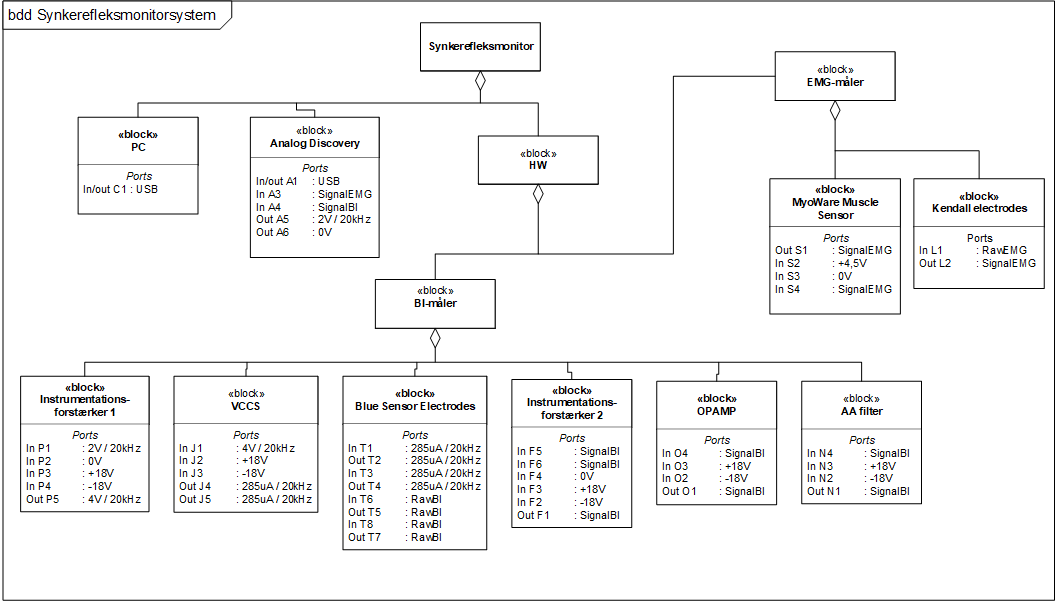
\includegraphics[width=\linewidth]
{Figure/BDD}}
\caption{Figuren viser de enkelte komponenter, som hardware-delen består af. Overordnet består systemet af en Bioimpedansmåler, en EMG-måler og enhed som både bruges til som dataopsamlingsenhed og funktionsgenerator. Udover det er der en PC blok.}
\label{figbdd}
\end{figure}

\section{Internal blok diagram}

Det interne blokdiagram på \ref{ibdfigur} viser den interne struktur og kommunikation mellem delsystemerne. Figur \ref{ibdfigur} indeholder to uafhængige blokke med navnene BI-måler og EMG-måler. De to blokke kommunikerer med Analog Discovery og en PC. For BI-målerens vedkommende starter kommunikationsflowet med at Analog Discovery'en generer et AC signal på 2V som sendes til den første af to Instrumentationsforstærker i BI-måler blokken. Instrumentationsforstærkeren forstærker de 2V med faktor 2. Det forstærkede signal sendes videre til strømgeneratoren, VCCS, som på baggrund af det indkommende 3V producerer en konstant strøm på. Strømmen sendes videre til et måleobjekt via. to elektroder, kaldet Blue Sensor Electrodes.  To yderligere elektroder påsættes på måleobjektet for at måle en spændingsforskel. Denne spændingsforskel er svag og kræver at blive forstærket. Denne forstærkning foregår over to trin. Til den første trin anvendes en instrumentationsforstærker efterfulgt af en operationsforstærker. Det forstærkede signal over de to trin sendes videre til et anti-aliaseringsfilter, der dæmper frekvenskomponenter over Nyquist-frekvensen. Tilslut sendes signalet til en dataopsamlingsenheden Analog Discovery, der sender det opsamlede signal videre til en PC for at blive analyseret og vist. Delsystemerne instrumentationsforstærker 1, 2 og AA filteret forsynes med en eksitationsspænding på $ \pm  $18V. \\

EMG-blokken består en Myoware Muscle Sensor og to elektroder, der måler spændingsfaldet over et valgt segment på et måleobjekt. Det målte signal opsamles også vha. Analog Discovery. Myoware Muscle Sensoren forsynes med en eksitationsspænding på 5V.  

\begin{figure}[H]
\centering
{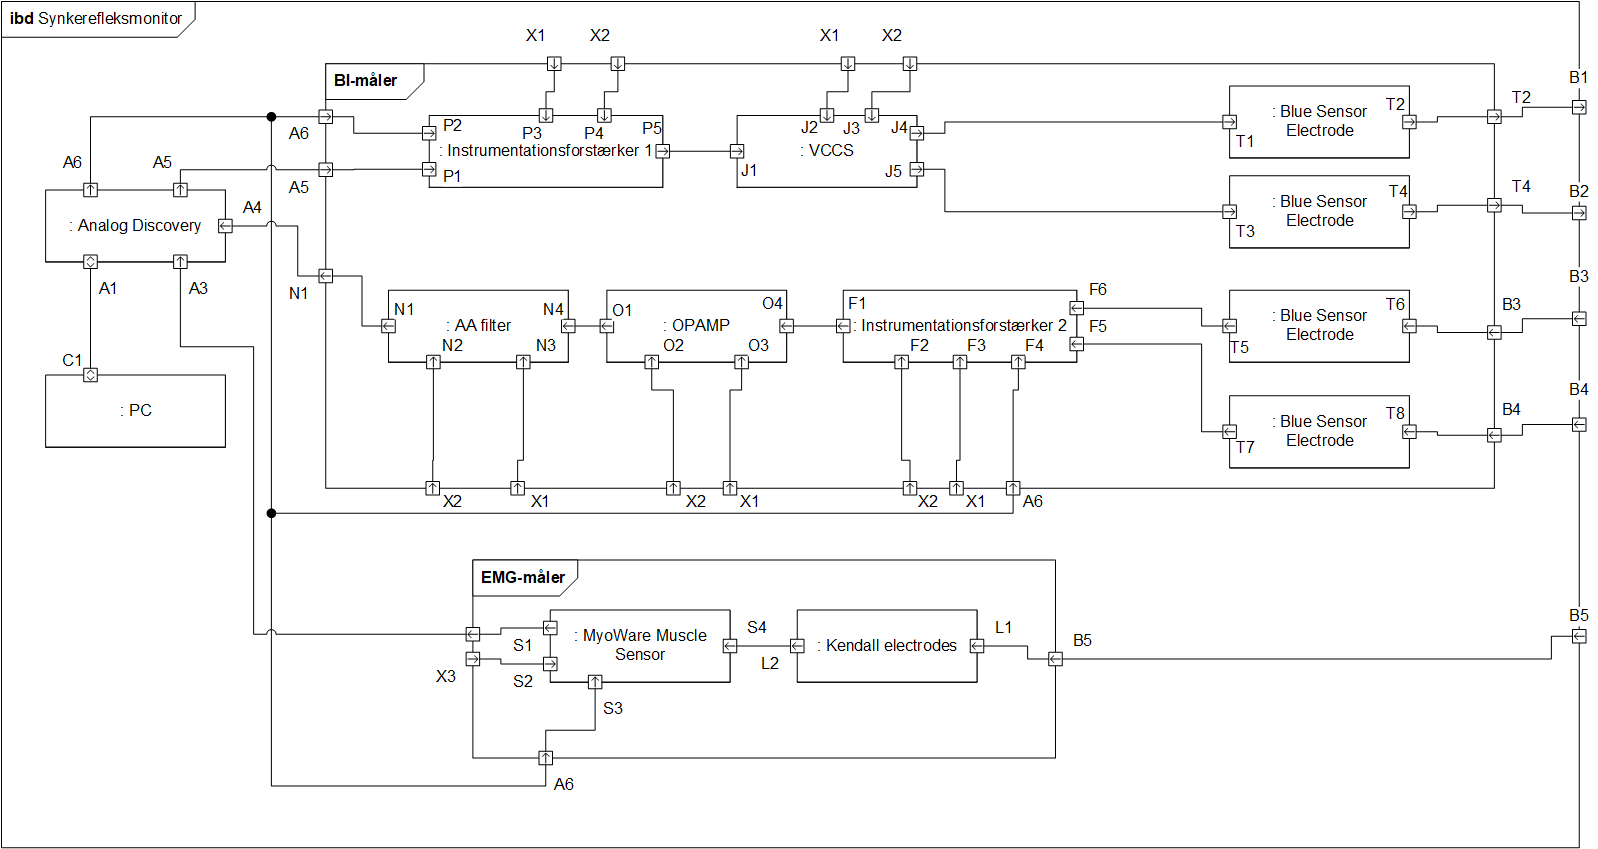
\includegraphics[width=\linewidth]
{Figure/IBD}}
\caption{Figuren viser et internt blokdiagram, der illustrer den interne relation og signalflow mellem delsystemer. Overordnet set indeholder diagrammet to hovedblokke med hver deres subkomponenter. Den ene af de store blokke repræsenter en bioimpedansmåler-apparat og den anden blok repræsenter en elektromyografi-apparat }
\label{ibdfigur}
\end{figure}

\section{Blokbeskrivelse} \label{blokbesk}
Nedenstående to tabeller viser hhv. grænsefladebeskrivelse og signalbeskrivelse af de blokke, som indgår i figur \ref{ibdfigur}.
\
\begin{table}[H]
\centering


\begin{tabular}{|p{4.3cm}|p{3.6cm}|p{2cm}|p{4cm}|}
\hline
\textbf{Blok-navn }                        & Funktionsbeskrivelse  & Signaler & Kommentar \\ \cline{3-4} \hline

PC & Behandler input fra Analog Discovery.  &  USB & Dataoverførelse med Analog Discovery   \\ \cline{3-4} \hline


Analog Discovery & Fungerer som funktionsgenerator, og  A/D-konverter. Den kommunikerer også med PC'en.  &  USB & Dataoverførelse med Analog Discovery   \\ \cline{3-4}

 	 
 	 &  & SignalEMG & Indgangssignal  \\ \cline{3-4}
 	 
 	 &  & SignalBI & Indgangssignal  \\ \cline{3-4}
 	 &  & $   ${2V,20kHz} & Funktionsgenerator  \\ \cline{3-4}
 	 &  & $   ${0V} & Reference  \\ \cline{3-4} \hline
 	 
 	 
Instrumentationsforstærker 1 & Forstærker 2V fra Analog Discovery til 4V.  &  $   ${2V,20kHz} & Ingangsspænding  \\ \cline{3-4}
&  & $   ${0V} & Funktionsgenerator  \\ \cline{3-4}
&  & $   ${+18V} & Eksitationsspænding   \\ \cline{3-4} 
&  & $   ${-18V} & Eksitationsspænding   \\ \cline{3-4} 
&  & $   ${2V,20kHz} & Udgangssignal   \\ \cline{3-4}  	  \hline


VCCS  & Genererer en konstant strøm.  &  $   ${4V,20kHz} & Ingangsspænding  \\ \cline{3-4}
&  & $   ${+18V} & Eksitationsspænding   \\ \cline{3-4} 
&  & $   ${-18V} & Eksitationsspænding   \\ \cline{3-4} 
&  & $   ${285uA,20kHz} & Udgangssignal   \\ \cline{3-4} \hline
 	 
Blue Sensor Electrodes & Transporterer strøm til et måleobjekt og måler biosignal fra et måleobjekt.
 &  $   ${285uA,20kHz} & Udgangssignal  \\ \cline{3-4}
&  & SignalBI & Indgangssignal   \\ \cline{3-4}  \hline 	 
 
 
Instrumentationsforstærker 2 &Forstærker biosignal fra et måleobjekt. 
&   SignalBI & Indgangssignal og udgangssignal  \\ \cline{3-4}
&  & $   ${0V} & Reference  \\ \cline{3-4}
&  & $   ${+18V} & Eksitationsspænding   \\ \cline{3-4} 
&  & $   ${-18V} & Eksitationsspænding   \\ \cline{3-4} 	\hline 
 	
OPAMP & Forstærker signalet fra instrumentationsforstærker 2. 
&   SignalBI & Indgangssignal og udgangssignal  \\ \cline{3-4}
&  & $   ${+18V} & Eksitationsspænding   \\ \cline{3-4} 
&  & $   ${-18V} & Eksitationsspænding   \\ \cline{3-4}  	 \hline


MyoWare Muscle Sensor & Behandler EMG input fra et måleobjekt. 
&   SignalEMG & Udgangssignal  \\ \cline{3-4}
&  & $   ${+5V} & Eksitationsspænding   \\ \cline{3-4} 
&  & $   ${0V} & Reference   \\ \cline{3-4}  	 \hline
 
 
Kendall electrodes & Transporterer biosignal fra et måleobjekt. 
&    RawEMG & Indgangssignal  \\ \cline{3-4}
&  & SignalEMG & udgangssignal   \\ \cline{3-4} 

 	 
\hline  
\end{tabular}
\caption{Figuren viser blokbeskrivelsen for systemmet synkerefleksmonitor} \label{BlokBeskr}
\end{table}

\pagebreak

% Please add the following required packages to your document preamble:
% \usepackage{multirow}
\begin{table}[H]
\centering
\caption{Figuren viser signalbeskrivelsen for systemet synkerefleksmonitor}
\label{my-label}
\begin{tabular}{|p{1.1cm}|p{2cm}|p{1.4cm}|p{3.5cm}|p{4.4cm}|p{2cm}|}
\hline

\textbf{Blok-navn}  & \textbf{Funktion}                                 & \textbf{Område} & \textbf{Port 1}      & \textbf{Port 2}                  & \textbf{Kommentar} \\ \cline{4-6} \hline


0V & Reference til analoge spændinger  &   & Analog Discovery, A6  & Instrumentationsforstærker 1, P2  &  stel   \\ \cline{4-6}

 &  &   &  Analog Discovery, A6 & Instrumentationsforstærker 2, F4 & \\ \cline{4-6} 
 
 &  &   &  Analog Discovery, A6 & MyoWare Muscle Sensor, S3 & \\ \cline{4-6}

 \hline
5V & Forsynings- spænding til MyoWare Muscle Sensor  &  4,9-5,1 V & Analog Discovery, A2 & MyoWare Muscle Sensor, S2&     \\ \cline{4-6}	\hline




+18V & Eksitations- spænding  &  16-18 V & X1& Instrumentationsforstærker 1, P3 &     \\ \cline{4-6}	

&  &   &  X1 & VCCS, J2 & \\ \cline{4-6} 
&  &   &  X1 & Instrumentationsforstærker 2, F3 & \\ \cline{4-6} 
&  &   &  X1 & OPAMP, O3 & \\ \cline{4-6} 
&  &   &  X1 & AA filter, N3 & \\ \cline{4-6} \hline

	
-18V & Eksitations- spænding  &  -16 - -18 V & X2& Instrumentationsforstærker 1, P4 &     \\ \cline{4-6}

&  &   &  X2 & VCCS, J3 & \\ \cline{4-6} 
&  &   &  X2 & Instrumentationsforstærker 2, F2& \\ \cline{4-6} 
&  &   &  X2 & OPAMP, O2 & \\ \cline{4-6} 
&  &   &  X2 & AA filter, N2 & \\ \cline{4-6}  \hline

 
 2V, 20kHz & Genererer AC signal på 20 kHz med en amplitude på 2V &  & Analog Discovery, A5& Instrumentationsforstærker 1, P1 &     \\ \cline{4-6} \hline

4V, 20kHz & Forstærket AC &  & Instrumentations- forstærker 1, P5& VCCS, J1 &     \\ \cline{4-6} \hline

285uA, 20kHz & Genereret strøm &  & VCCS, J4 &Blue Sensor Electrode, T1 &     \\ \cline{4-6} 

&  &   &  VCCS, J5 & Blue Sensor Electrode, T3 & \\ \cline{4-6} \hline

Signa- lBI & Biosignal fra måleobjekt  & & Blue Sensor Electrodes, T5& Instrumentationsforstærker 2, F6 &     \\ \cline{4-6}

&  &   &  Blue Sensor Electrodes, T7 &Instrumentationsforstærker 2, F6 & \\ \cline{4-6} 
&  &   &  Instrumentations forstærker 2, F1 & OPAMP, O4& \\ \cline{4-6} 
&  &   &  OPAMP, O1 & AA filter, N4 & \\ \cline{4-6} 
&  &   &  AA filter, N1 & Analog Discovery, A4 & \\ \cline{4-6}  \hline


Signal- EMG& EMGsignal fra måleobjekt &  & IMyoWare Muscle Sensor, S1, P5& Analog Discovery, A3 &     \\ \cline{4-6} \hline

USB& Kommunikation med Analog Discovery &  & PC, C1& Analog Discovery, A1 &     \\ \cline{4-6} \hline

\end{tabular}
\end{table}

\chapter{Software} \label{swafsnit}
\section{Blok definition diagram}

Dette afsnit omhandler arkitekturen af   softwaren, som anvendes til analysering og visning af bioimpedans- og EMG-målinger. Arkitekturen af softwaren er drevet af de usecases, som er beskrevet i afsnittet systembeskrivelse. På baggrund af disse usecases udformes et BDD, som indeholder en parent-blok og to child-blokke, der hver indeholder funktioner/metoder.
I dette projekt anvendes  Matlab til at realisere projektets  software-del.  Funktionaliteter som ønskes implementeret i Matlab kodes som funktioner. Disse funktioner skrives hver i en selvstændig script-fil, som kaldes fra en GUI fil, når de skal bruges. Da det ønskes i dette projekt at implementere en Matlab GUI med kontroller skrives koden til disse kontroller i funktioner. Kontrollerne kan være en knap, tekstfelt eller tekstboks. I stedet for at kode alle funktioner i én scriptfil tildeles hver funktionen sin egen scriptsession. Hver scriptsession udfører en bestemt opgave, samt kan interagere med andre funktion. Konkret fungerer softwaren ved at et sundhedspersonale initialiserer kodeeksekveringen ved at starte programmet Synkerefleksmonitor og efterfølgende trykke knappen ’Start measurments'. Denne initiering af sundhedspersonalet medfører at der foretages to målinger simultant. Disse målinger analyseres og vises til sundhedspersonalet. Rækkefølgen hvori programmets kode eksekveres beskrives vha. et sekvens diagram. Dette diagram kan læses i designbilaget.    


\begin{figure}[H] 
\centering
{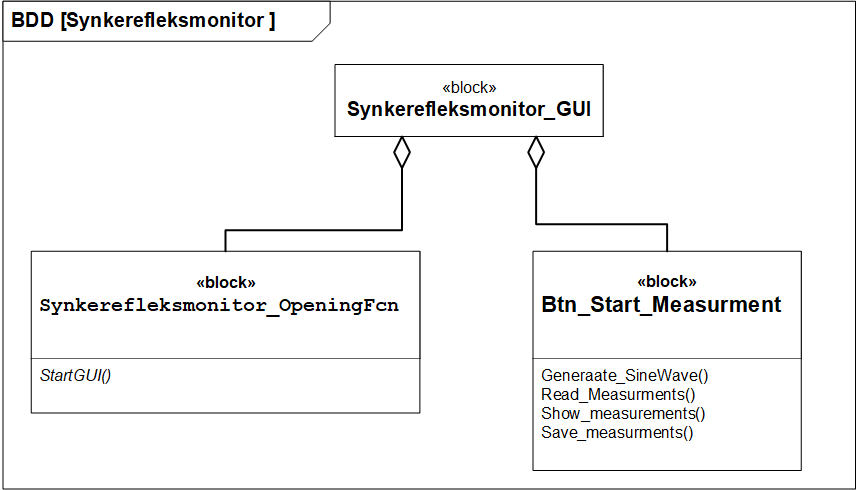
\includegraphics[width=\linewidth]
{Figure/SWIBD}}
\caption{Figuren viser block definition diagrammet for det ønsket software. Diagrammet indeholder en hovedblok, der består af to andre bl  okke, som hver indeholder Matlab funktioner. Disse funktioner tilsammen analyserer og viser to målinger simultant  }
\label{figScrip}
\end{figure}

\textbf{USE casene skal ændres der vi nu har en anderledes sw arkitektur}

\citep{Aroom2009}
\bibliography{library}
\end{document}